\section{Actividad 1: Polarización de la juntura BE}

\paragraph{Armar el circuito en una plataforma de simulación con el objetivo de observar la curva de la corriente de base a medida que aumenta la tensión de polarización de la juntura base-emisor. Es importante identificar el codo de la corriente y la estabilidad de la tensión VBE una vez polarizada la juntura. Podría, sí le parece, hacer simulaciones modificando otros parámetros que en el circuito básico se encuentran fijos como VCC(V2) o la temperatura ambiente simulada.}



\subsection{Materiales usados:}
\begin{itemize}
    \item Transistor BC546/7/8/9.
    \item Resistores $R_s = \SI{10}{\kilo\ohm}$, $R_c = \SI{560}{\ohm}$.
    \item Fuentes de alimentación.
\end{itemize}


\subsection{Mediciones:}
Mantenemos la $V_{CC} = 10V$, realizamos un barrido de 0V a 10V de $V_{BB}$ para completar la siguiente tabla:

\begin{table}[H]
    \centering
    \resizebox{0.49\textwidth}{!}{%
    \begin{tabular}{|c|c|c|c|c|c|c|}
        \hline
        $V_{BB}$ & 500mV & 1V & 2V & 3V & 4V & 10V \\
        \hline
        $I_B$    &   $4,5\mu A$    &  $30,43\mu A$  &  $124 \mu A$  &  $220 \mu A$  &  $323 \mu A$  &  $913 \mu A$   \\
        \hline
        $V_{BE}$ &    $0,493V$   &  $0,682V$  &  $0,73V$  &  $0,74V$  &  $0,74V$  &   $0,75V$  \\
        \hline
    \end{tabular}
    }
    \caption{Tabla 1}
    \label{tab:mediciones}
\end{table}

\begin{figure}[H]
    \centering
    \resizebox{0.49\textwidth}{!}{%
    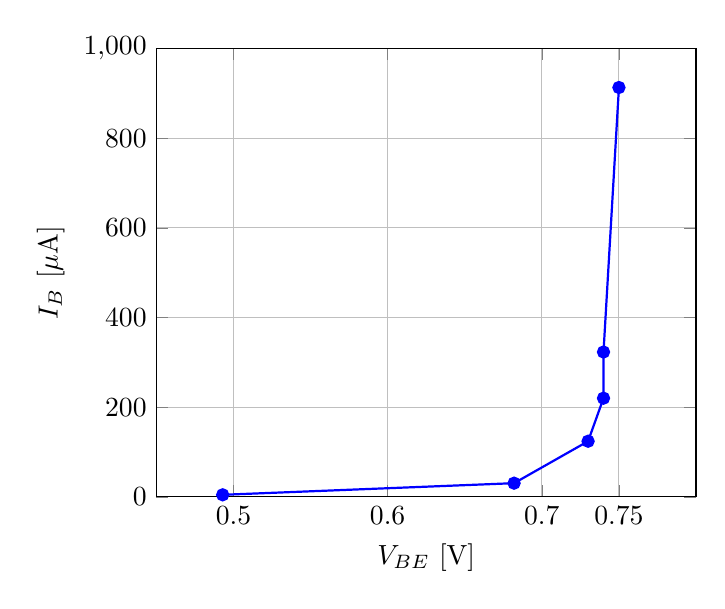
\begin{tikzpicture}
        \begin{axis}[
            xlabel={$V_{BE}$ [V]},
            ylabel={$I_B$ [$\mu$A]},
            grid=both,
            xmin=0.45, xmax=0.8,
            ymin=0, ymax=1000,
            xtick={0.5,0.6,0.7,0.75},
            ytick={0,200,400,600,800,1000},
            legend pos=north west,
        ]
        \addplot[
            color=blue,
            mark=*,
            thick
        ] coordinates {
            (0.493,4.5)
            (0.682,30.43)
            (0.73,124)
            (0.74,220)
            (0.74,323)
            (0.75,913)
        };
        \end{axis}
    \end{tikzpicture}
    }
    \caption{Curva de $I_B$ en función de $V_{BE}$}
    \label{fig:ib_vs_vbe}
\end{figure}
